\documentclass{beamer}

\usefonttheme{professionalfonts} % using non standard fonts for beamer
\usefonttheme{serif} % default family is serif

\usepackage{enumitem}
\setitemize{label=\usebeamerfont*{itemize item}%
  \usebeamercolor[fg]{itemize item}
  \usebeamertemplate{itemize item}}

\usepackage{hyperref}
\usepackage{booktabs}
\usepackage{xfp}
\usepackage{graphicx}
\def\Put(#1,#2)#3{\leavevmode\makebox(0,0){\put(#1,#2){#3}}}
\usepackage{colortbl}
\usepackage{tikz}
\usepackage{amssymb}
\usepackage{enumerate}
\usepackage{arydshln}
\usepackage{algorithm}
\usepackage{algpseudocode}
\usepackage{subcaption} %to have subfigures available

\usepackage[absolute,overlay]{textpos}

\colorlet{lightred}{red!25}
\colorlet{lightgreen}{green!25}
\beamertemplatenavigationsymbolsempty

\newcommand\blfootnote[1]{%
  \begingroup
  \renewcommand\thefootnote{}\footnote{#1}%
  \addtocounter{footnote}{-1}%
  \endgroup
}

\makeatletter

%% Textclass specific LaTeX commands.
\newcommand\makebeamertitle{\frame{\maketitle}}%
\AtBeginDocument{%
  \let\origtableofcontents=\tableofcontents
  \def\tableofcontents{\@ifnextchar[{\origtableofcontents}{\gobbletableofcontents}}
  \def\gobbletableofcontents#1{\origtableofcontents}
}
%% User specified LaTeX commands.
\usetheme{Malmoe}
\useoutertheme{infolines}
\addtobeamertemplate{headline}{}{\vskip2pt}
\setbeamercovered{transparent}

\title[PFlock report]{PFLOCK Report}
\author[AC]{Andres Calderon}
\institute[UCR]{University of California, Riverside}
\makeatother

%%%%%%%%%%%%%%%%%%%%%%%%%%%%%%%%%%%%%%
%% Main document
%%%%%%%%%%%%%%%%%%%%%%%%%%%%%%%%%%%%%%
\begin{document}
\makebeamertitle
\newif\iflattersubsect

\AtBeginSection[] {
    \begin{frame}<beamer>
    \frametitle{Outline} 
    \tableofcontents[currentsection]  
    \end{frame}
    \lattersubsectfalse
}

\AtBeginSubsection[] {
    \begin{frame}<beamer>
    \frametitle{Outline} 
    \tableofcontents[currentsubsection]  
    \end{frame}
}

\begin{frame}{Candidate pruning bottleneck...}{We have to deal with +188K candidates...}
    \centering
    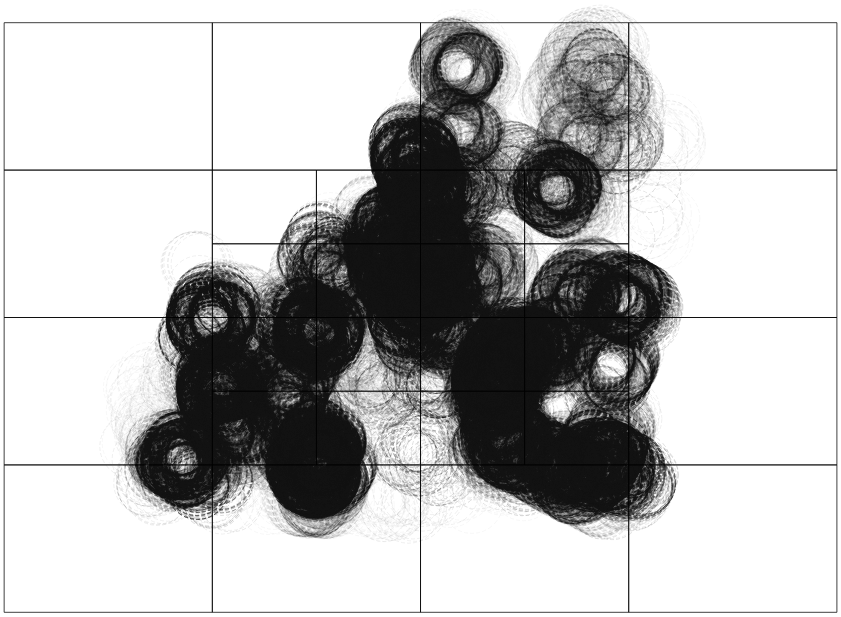
\includegraphics[width=0.6\textwidth]{figures/candidates}
\end{frame}

\begin{frame}{Candidate pruning bottleneck...}{$\varepsilon=20$ and $\mu=3$}
    \centering
    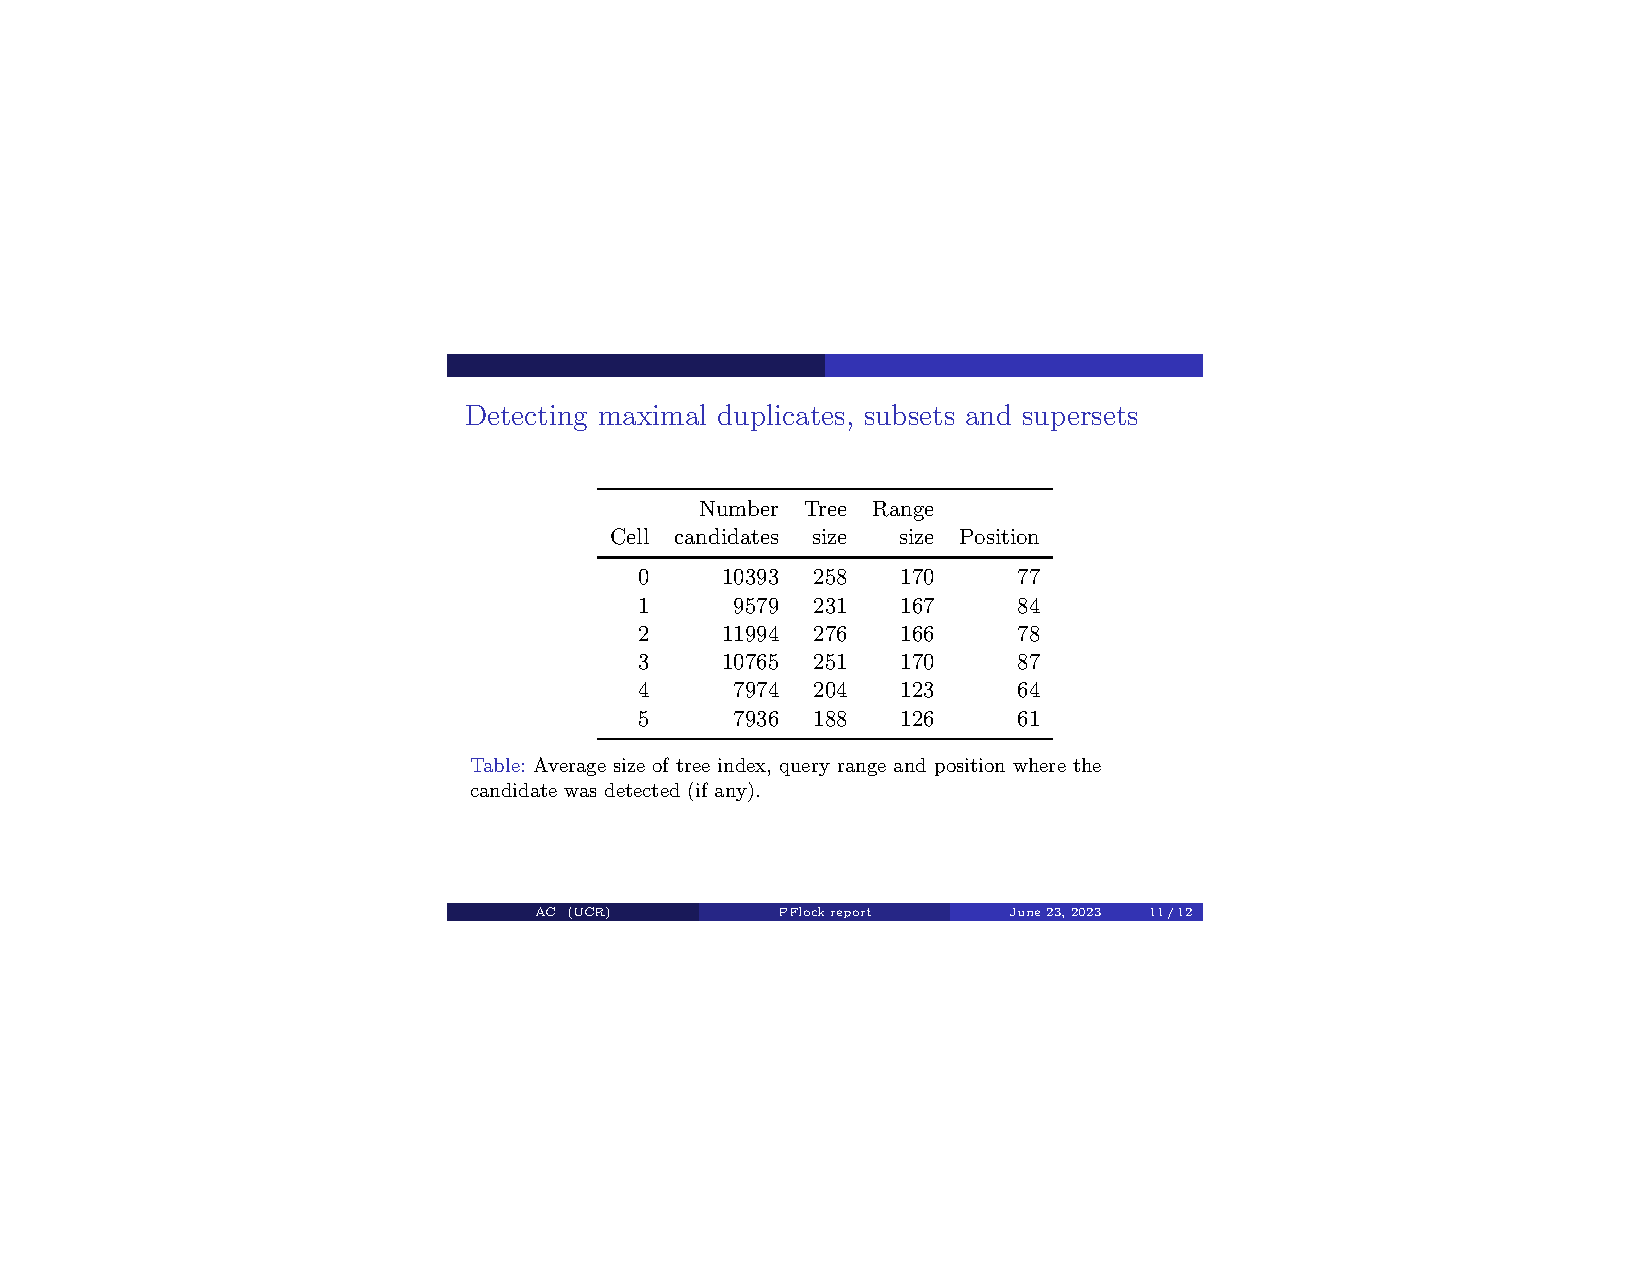
\includegraphics[trim=8cm 9cm 8cm 8cm, clip, width=\textwidth]{figures/table}
    Indeed...
    \begin{itemize}
            \item Average size of maximal disks hold in the tree: 25.88
            \item Average size of candidate disks query to the tree: 17.70
    \end{itemize}
\end{frame}

\begin{frame}{Currently working on PSB \textrightarrow PSI...}{Plane sweeping [80\%]}
    \centering
    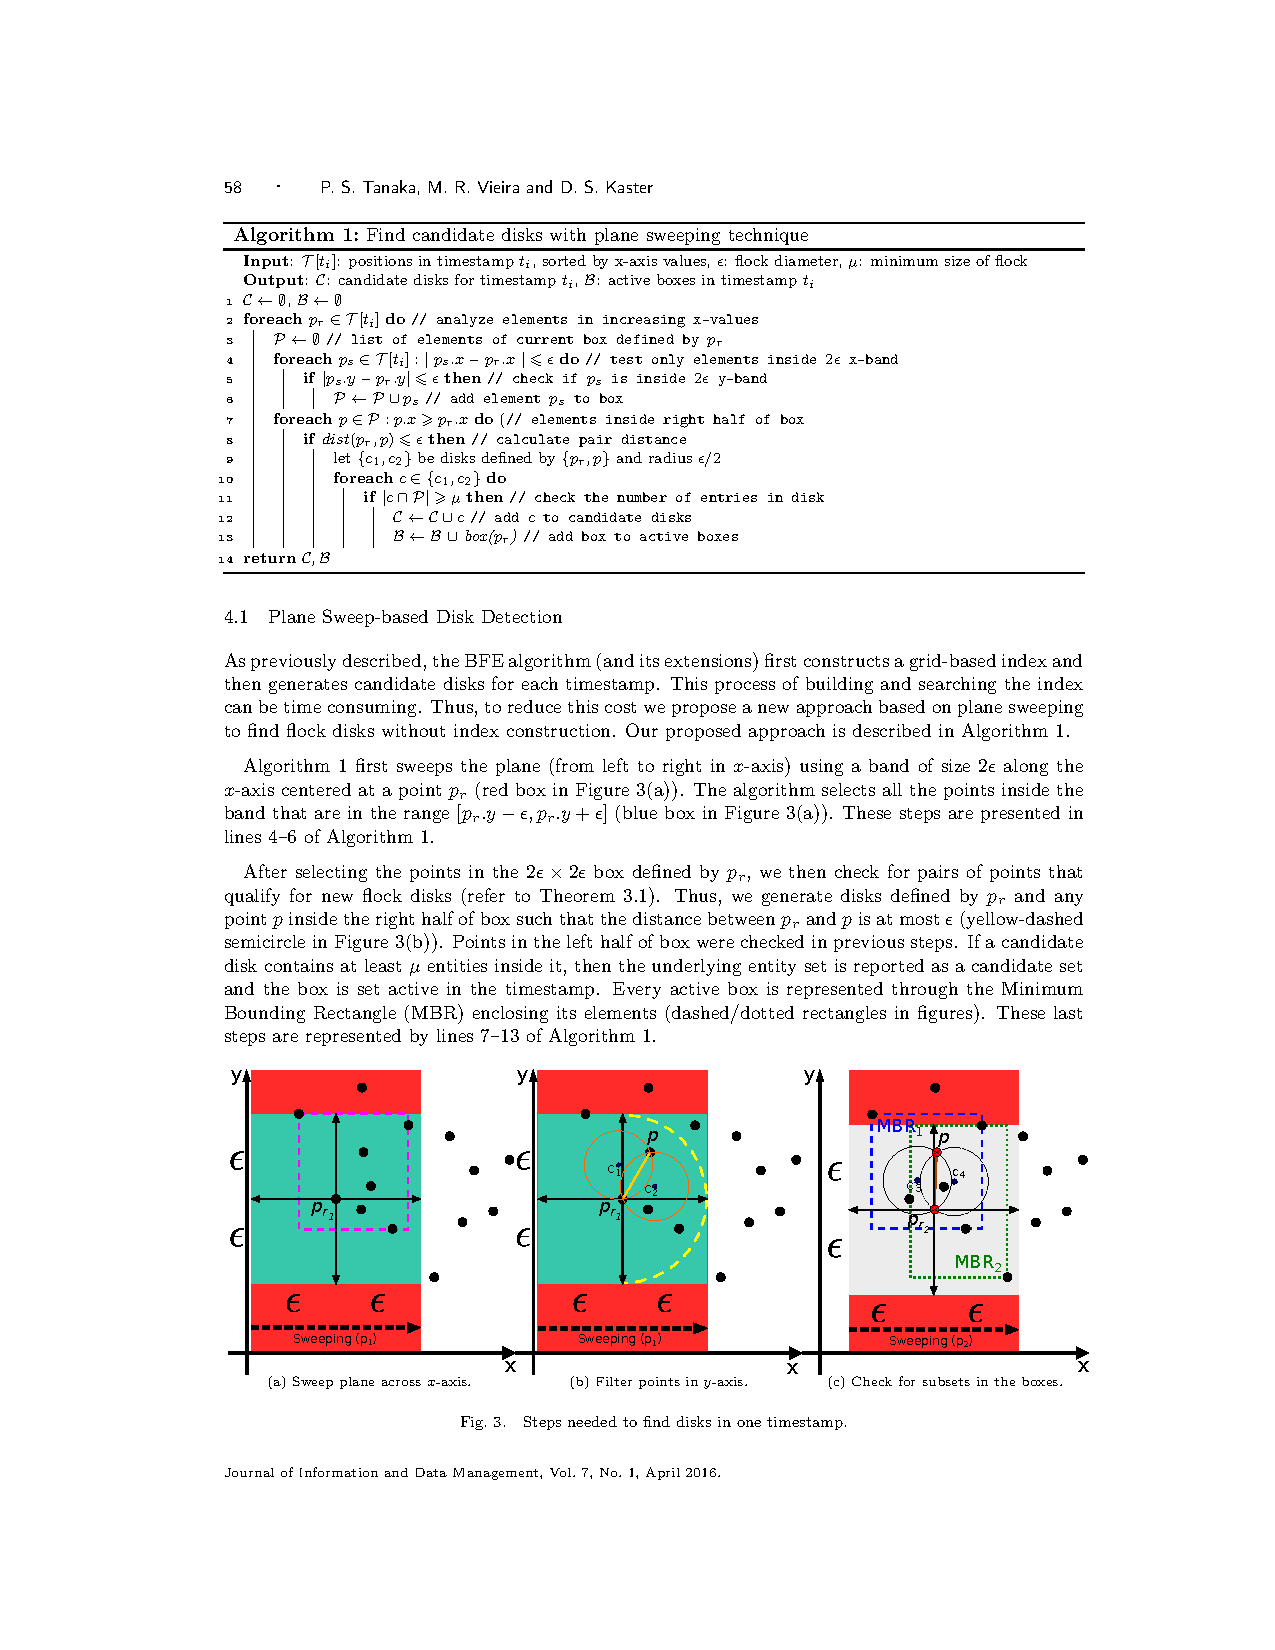
\includegraphics[trim=3.5cm 4.25cm 3.15cm 18cm, clip, width=0.9\textwidth]{figures/sweeping}
    %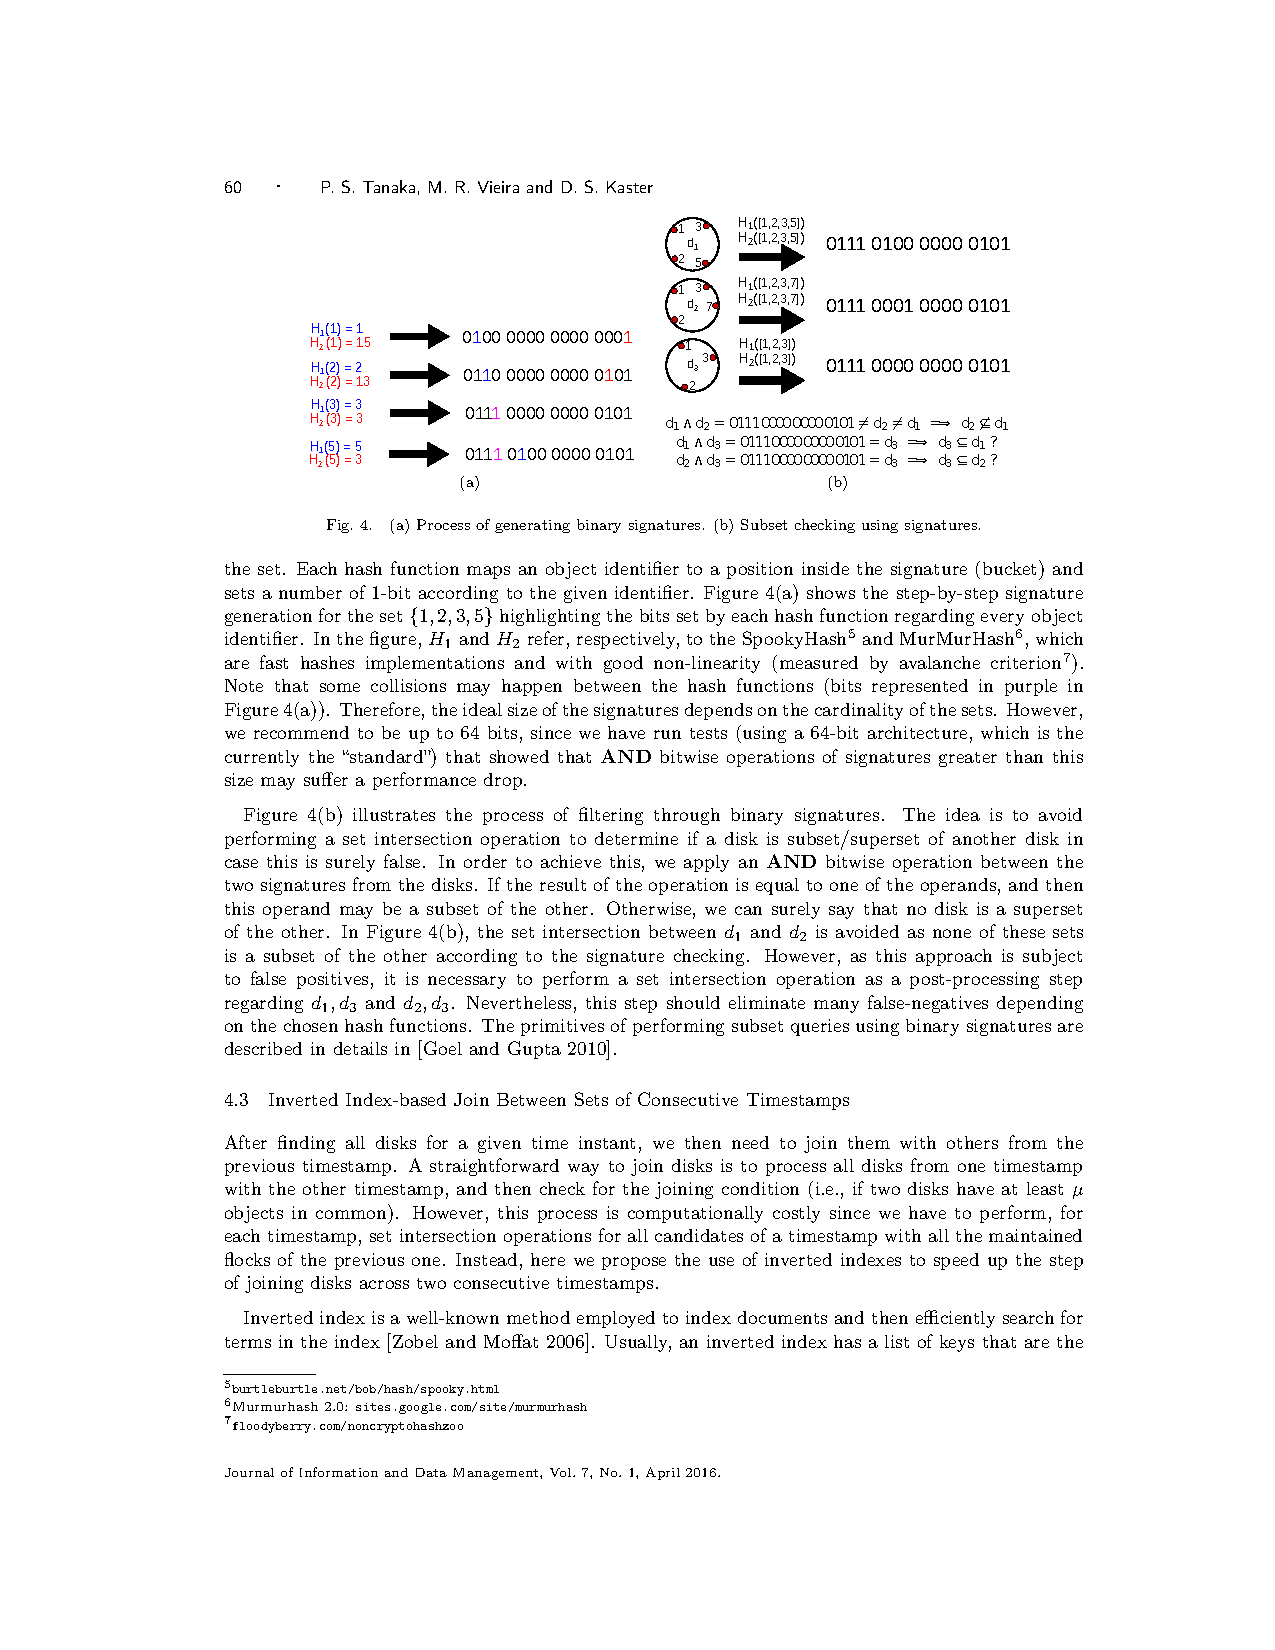
\includegraphics[trim=8cm 9cm 8cm 8cm, clip, width=\textwidth]{figures/signatures}
\end{frame}

\begin{frame}{Currently working on PSB \textrightarrow PSI...}{Binary signature [50\%]}
    \centering
    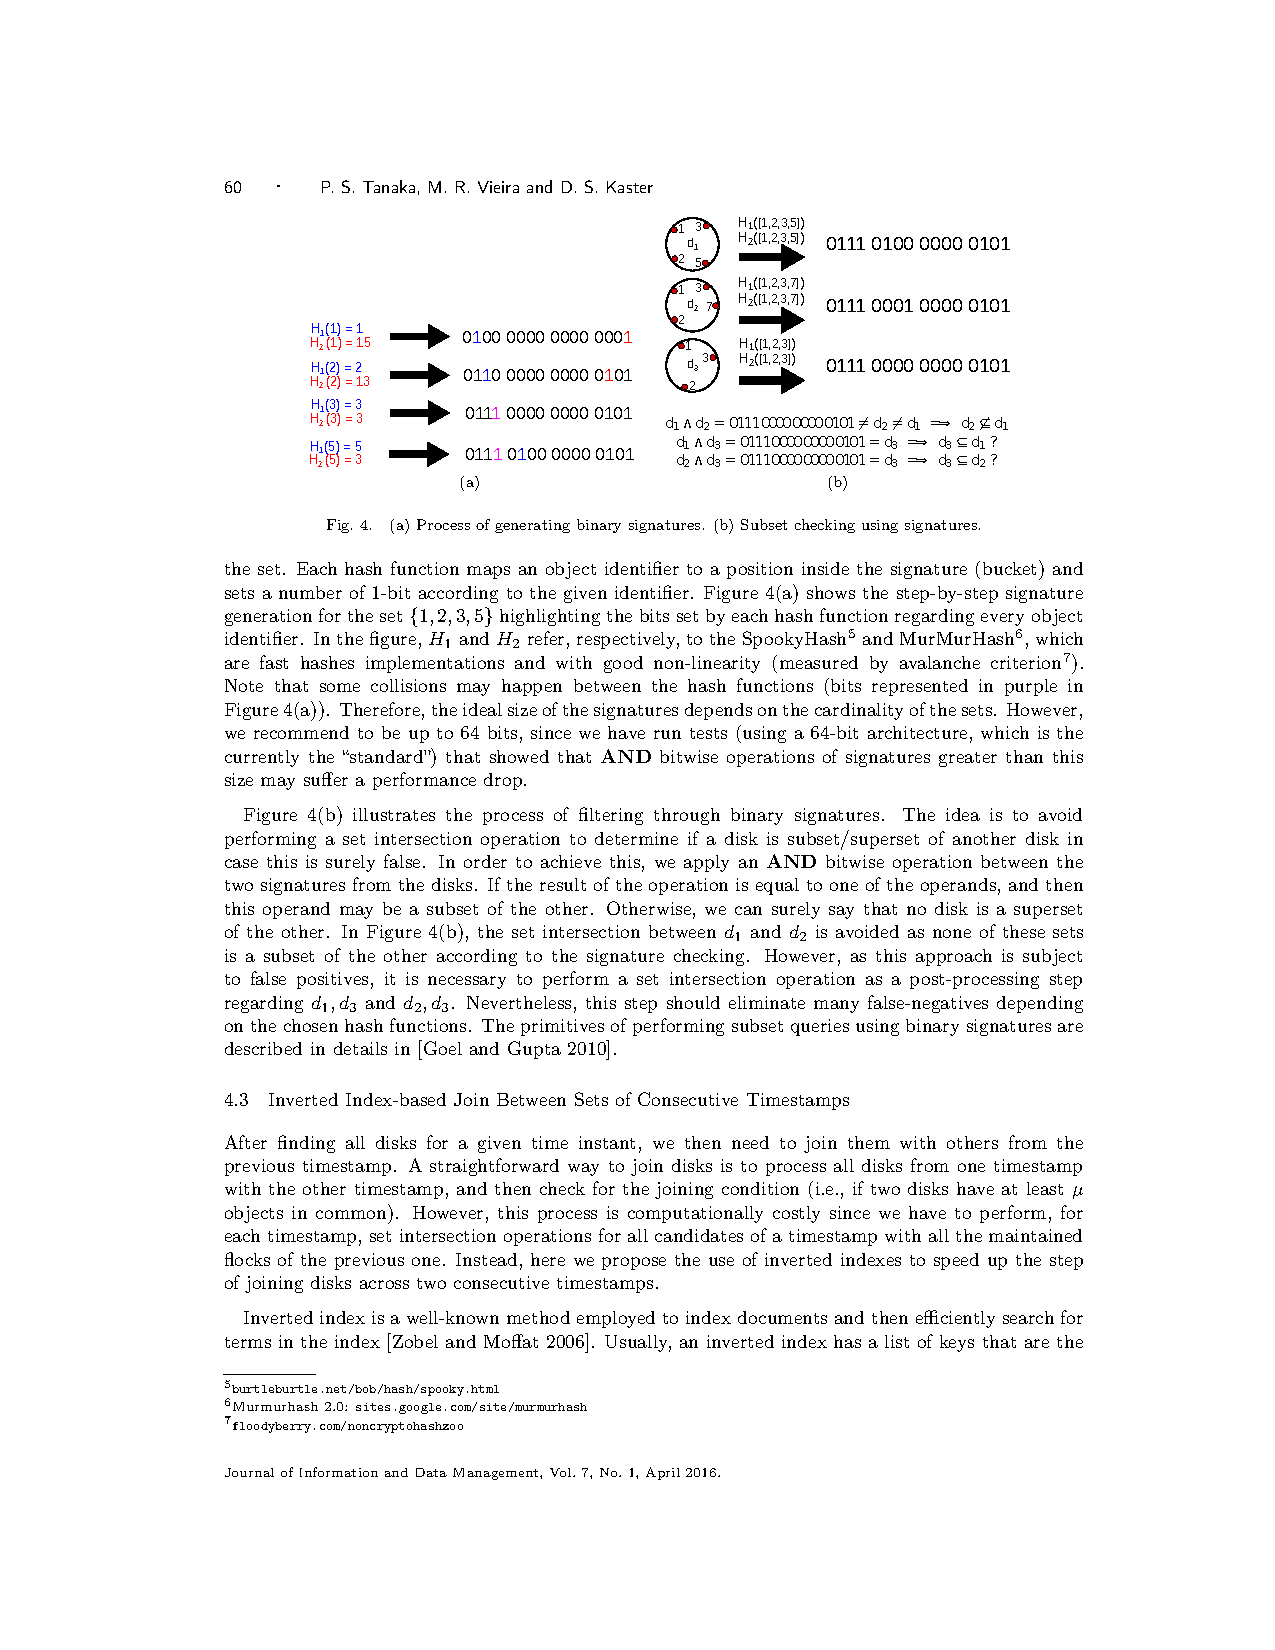
\includegraphics[trim=4.75cm 19.95cm 4cm 3.5cm, clip, width=\textwidth]{figures/signatures}
\end{frame}

\begin{frame}{Alternative trajectory datasets...}{ny\_bikes [\href{https://citibikenyc.com/system-data}{Citi Bike NY}]}
    \centering
    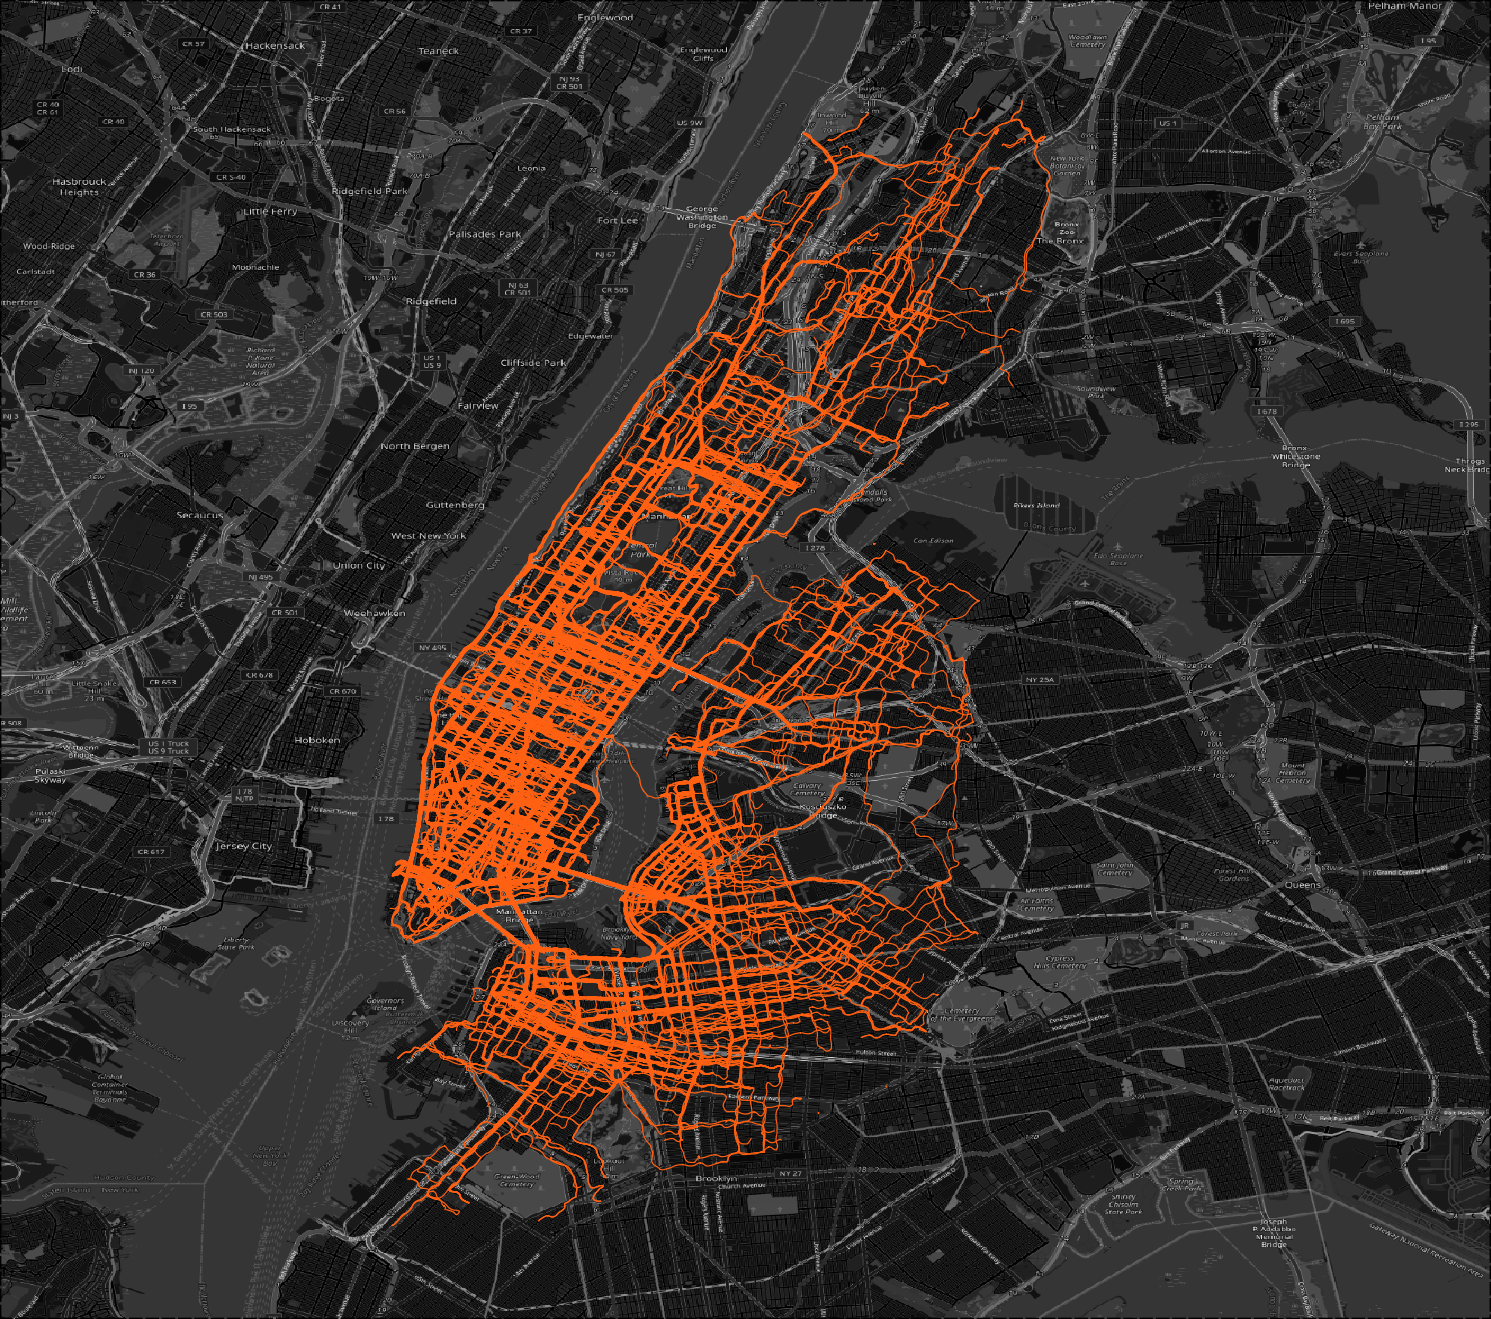
\includegraphics[width=0.625\textwidth]{figures/ny_bikes}
    \begin{tabular}{r r}
            \small Trajectories: 2'734.157 & \small Time span: March 2023
    \end{tabular}
\end{frame}

\begin{frame}{Alternative trajectory datasets...}{ny\_taxis [\href{https://chriswhong.com/open-data/foil_nyc_taxi/}{TLC Trip Record Data}]}
    \centering
    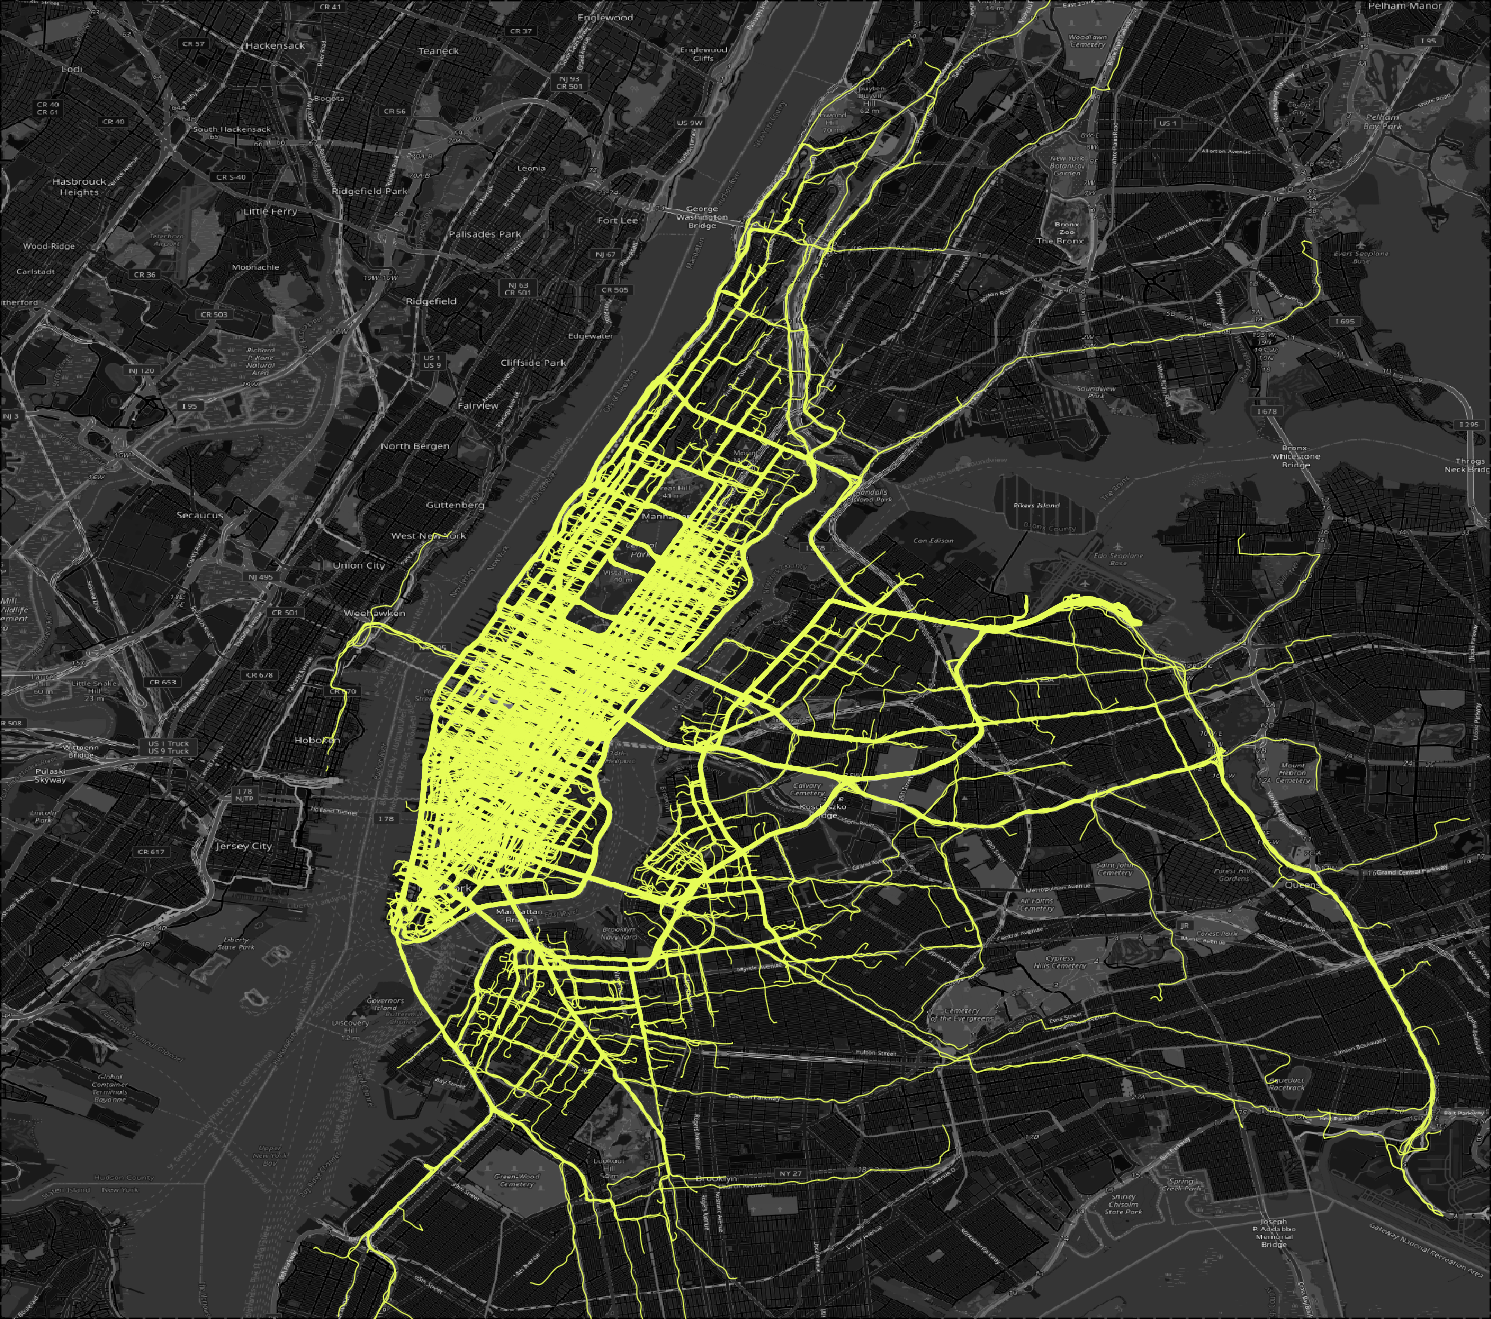
\includegraphics[width=0.625\textwidth]{figures/ny_taxis}
    \begin{tabular}{r r}
            \small Trajectories: 14'336.486 & \small Time span: October 2013
    \end{tabular}
\end{frame}

\begin{frame}{What's next?}
  \begin{itemize}
          \item Complete implementation for PSB (plane sweeping and binary signatures)...
          \item Run interpolation for new datasets...
          \item Start working on temporal dimension...
          \begin{itemize}
                  \item Explore 3D partitioners...
          \end{itemize}
  \end{itemize}

\end{frame}

\end{document}

